% TC:group tabular 1 1
% TC:group table 1 1

\definecolor{bblue}{HTML}{4F81BD}
\definecolor{rred}{HTML}{C0504D}
\definecolor{ggreen}{HTML}{9BBB59}
\definecolor{ppurple}{HTML}{9F4C7C}
\definecolor{yyellow}{HTML}{CCAA40}
\definecolor{bbrown}{HTML}{662233}
\definecolor{excelGreen}{HTML}{50AA45}
\definecolor{sibPurple}{HTML}{822689}

\newcommand{\mycbox}[1]{\tikz{\path[draw=#1,fill=#1] (0,0) rectangle (0.3cm,0.3cm);}}

\chapter{Evaluation}

\paragraph{} This chapter discusses the Excello implementation effectiveness with regards to the success criteria and by showcasing examples. The conversion of MIDI corpora to the Excello notation using the converter demonstrates the expressiveness of the notation. Next the summative evaluation is explained and its data used to assess the features implemented in the participatory design process and to reason about Excello using the CDN framework \cite{blackwell:tutorial}. Finally, the ethics and data handling procedures shall be covered.

\section{Excello Success}

\paragraph{} Both a musical notation and corresponding program integrated into Excel for playback have been implemented. As required by the success criteria, users can play multiple notes and chords of different durations. These can be combined into looped sequences and have defined tempo. In the participatory design process additional features were added as extensions; defining multiple successive notes in a cell, turtles calculating how far they should move and nested instructions with repeats are additional features facilitating more efficient notation. Custom Excel functions, a chord adding tool and faster turtle toggling allows users to work more efficiently. Figure \ref{evaluation:excelloFranzRedacted} shows Excello in use with a participant's arrangement.

\begin{figure}[tbh]
\centerline{\includegraphics[width=150mm]{figs/excelloFranzRedacted.png}}
\caption{An arrangement with separated and labelled parts per instrument. Turtles refer to a global tempo at the top of the spreadsheet.}
\label{evaluation:excelloFranzRedacted}
\end{figure}

\paragraph{} The first section of Reich's Piano Phase is two equal piano melodies, one played slightly faster than the other. The two parts move out of phase periodically aligning at different offsets. This is included as an example for many end-user programming tools. This is implemented in Manhattan using three rows of 24 columns \cite{nash:manhattan}. Sonic Pi requires one line for the notes and eight for playback. Piano Phase can not be concisely notated by western staff notation. Excello only requires two cells to define two turtles of different speeds in addition to the notes. All three implementations are shown in figure \ref{evaluation:phase}.

\begin{figure}[ht]
\begin{tabular}{cc}
  \multirow{3}{*}[2.72cm]{\includegraphics[width=65mm]{figs/manhattanPhase.png}} & \includegraphics[width=65mm]{figs/sonicPiPhase.png} \\
  & (b) The defined notes are played\\
  & by two concurrent loops with\\
  & different gaps between each note.\\[6pt]
  (a) Column 01 keeps track of the phase,& \multirow{2}{*}{\includegraphics[width=65mm]{figs/excelloPhase.png}} \\
  02 defines the notes and 03 is the &\\
  phased notes - defined with formulae &\\
  that update depending on the phase and& (c) Two turtles play the same\\
  defined notes.& notes at different speeds.\\
\end{tabular}
\caption{Implementations of Steve Reich's Piano Phase in a) Manhattan, b) Sonic Pi, c) Excello}
\label{evaluation:phase}
\end{figure}

\section{MIDI Corpus Conversion}

\paragraph{} Whilst being able concisely notate music western notation and other end-user programming systems can not, Excello can exactly express piece defined in MIDI. If tempo is redefined within a track, this is not be accounted for. If instead the time between messages is adjusted, the uncompressed file will account for this but the compressing algorithms will produce erroneous results as the difference between notes deviate too far from non-integer multiples of the minimum. Instrument specific effects such as piano pedals are not supported. Provided the difference between any two notes is a multiple of the minimum difference, the compression method that divides by this amount accurately reproduces the music, whilst resulting in spreadsheets orders of magnitude smaller. This method would not accurately convert quavers against triplets (three notes played in the same time as two) provided these notes were not multiples of a smaller note. Given the lengths of MIDI notes can be different to the space the note occupies in standard notation, an assumption on the ratio of note lengths was required for a more compressive conversion. The modal compressive conversion is lossy if the minimum note distance is not the modal distance. This is useful if there are ornaments or notes within a piece that dramatically decrease the minimum distance but occur infrequently. Therefore this loss may be useful for more efficient representations.

\paragraph{} I have converted three MIDI corpora. A collection of 497 Bach chorales\footnote{Accessed from https://github.com/jamesrobertlloyd/infinite-bach/tree/master/data/chorales/midi} made by Margaret Greentree, 280 piano pieces\footnote{http://piano-midi.de/midis.htm} held by Bernd Krueger under a creative commons license, and 194 Bach pieces made available from ``A Johann Sebastian Bach Midi Page"\footnote{http://www.bachcentral.com/midiindex.html}. This is not all the files available from this site as some were not readable by the python MIDI reader. All 971 MIDI files were converted using all three methods.

\paragraph{} The language of Excello is expressive enough to represent MIDI files and can do so concisely provided the condition of minimum note onset differences is maintained.

\section{Summative Evaluation Sessions}

\paragraph{} 19 Of the 21 users who participated in formative evaluation continued using Excello so could answer a summative evaluation questionnaire. First a review of the features that had been added since the initial sessions was given. To ensure users had a sufficient understanding of the interface before giving feedback, a short transcription task also requiring some authoring was given.

\paragraph{} The questionnaire first evaluated the features added during the participatory design process by comparing the interface before and after a feature had been added. Questions tested if the issues had been solved and if overall the change rendered the system more preferable. These were answered using a seven-point Likert scale. The remaining questions were based on Blackwell and Green's CDN questionnaire \cite{blackwell:questionnaire}. CDN can be used to analyse musical notation \cite{blackwell:notation} in addition to software systems \cite{green:cdn}, therefore it is suitable for the discussion of the Excello notation and interface. Dimensions significance for different activities varies \cite{blackwell:tutorial}, so users identified the percentage of time they spent carrying out these activities (searching for information, translating, incrementation, modification and exploratory design). Likert scale questions focusing on closeness of mapping, consistency, secondary notation, viscosity and visibility were used as planned in the proposal. It was suspected that reasoning about cognitive dimensions would be more challenging for participants, so to reduce the expected variance, only a five-point Lichard scale was used. In addition the two have been shown to produce similar results \cite{dawes:points}. CDN results were also collected for the user's preferred music composition interface. 12 users chose Sibelius, which shall be used for comparison.

\section{Success of Participatory Design}

\paragraph{} For each feature added, Excello with (system 2) and without this feature were compared. The following charts show the frequency of Likart scale responses for each question. I considered the mode of the Likert scale \cite{barry:likert}. Chi-squared goodness-of-fit test confirm the distributions are significantly different to uniform. As all expected values must be greater than 1 and 80\% greater than or equal to five \cite{ross:introductory} and the expected frequency for one result is $19/7 \approx 2.7$, I combine Strongly Disagree with Disagree, Strongly Agree with Agree and the remaining three options into a third group. The p-value from a chi-squared test with these three categories is given.

\subsection{Dynamics in the Cell}

\begin{table}[!htbp]
\centering
% \caption{Grammar rules for turtle movement instructions. $z \in \mathbb{Z}, n \in \mathbb{N}, c \in \texttt{[A-Za-z]}^{+}$.}
\vspace{1pt}
\begin{tabular}{|l|l|l|} \hline
\textbf{Statement}&\textbf{Mode}&\textbf{p-value}\\ \hline
\mycbox{bblue} It is easier to figure out the turtles path.&Strongly Agree&0.0000\\ \hline
\mycbox{rred} It is easier to figure out what dynamics different&Strongly Agree&0.0146\\
notes are played at.&&\\ \hline
\mycbox{ggreen} It is easier to tell the order in which dynamics are applied.&Strongly Agree&0.0000\\ \hline
\mycbox{ppurple} It is easier to write dynamics in the correct place.&Strongly Agree&0.0000\\ \hline
\mycbox{yyellow} Overall system 2 is preferable.&Strongly Agree&0.0000 \\ \hline
\end{tabular}
\label{evaluation:cellDynamics}
\end{table}

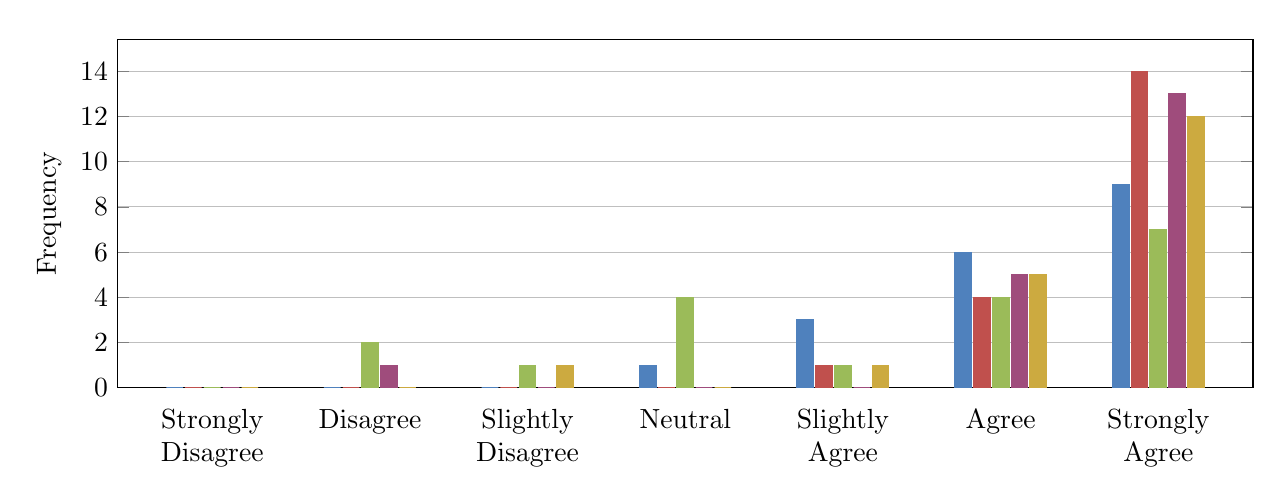
\begin{tikzpicture}
    \begin{axis}[
      % width  = \textwidth,
      width = 16cm,
      height = 6cm,
      major x tick style = transparent,
      ybar=2*\pgflinewidth,
      bar width=6pt,
      ymajorgrids = true,
      ylabel = {Frequency},
      %xlabel = {Likert Scale Result},
      symbolic x coords= {-3,-2,-1,0,1,2,3},
      xticklabels = {Strongly Disagree,Disagree,Slightly Disagree,Neutral,Slightly Agree,Agree,Strongly Agree},
      xtick = data,
      ytick = {0,2,4,6,8,10,12,14},
      x tick label style  = {text width=2cm,align=center},
      scaled y ticks = false,
      % enlarge x limits=0.25,
      ymin=0,
      legend cell align=left,
      legend style={
              at={(1,1.05)},
              anchor=south east,
              column sep=1ex
      }
    ]
        \addplot[style={bblue,fill=bblue,mark=none}]
            coordinates {(-3,0) (-2,0) (-1,0) (0,1) (1,3) (2,6) (3,9) };

        \addplot[style={rred,fill=rred,mark=none}]
             coordinates {(-3,0) (-2,0) (-1,0) (0,0) (1,1) (2,4) (3,14) };

        \addplot[style={ggreen,fill=ggreen,mark=none}]
             coordinates {(-3,0) (-2,2) (-1,1) (0,4) (1,1) (2,4) (3,7) };

        \addplot[style={ppurple,fill=ppurple,mark=none}]
             coordinates {(-3,0) (-2,1) (-1,0) (0,0) (1,0) (2,5) (3,13) };

       \addplot[style={yyellow,fill=yyellow,mark=none}]
           coordinates {(-3,0) (-2,0) (-1,1) (0,0) (1,1) (2,5) (3,12) };

        % \legend{It is easier to figure out the turtles path,It is easier to figure out what dynamics different notes are played at,It is easier to tell the order in which dynamics are applied,It is easier to write dynamics in the correct place,Overall system 2 is preferable}
    \end{axis}
\end{tikzpicture}

\paragraph{} There is strong evidence to suggest this change improved some of the issues identified during participatory design, resulting in an improved system.

\subsection{Inferred Octave}
\ %This is here to put the section heading and table in the right order

\begin{table}[!ht]
\centering
% \caption{Grammar rules for turtle movement instructions. $z \in \mathbb{Z}, n \in \mathbb{N}, c \in \texttt{[A-Za-z]}^{+}$.}
\vspace{1pt}
\begin{tabular}{|l|l|l|} \hline
\textbf{Statement}&\textbf{Mode}&\textbf{p-value}\\ \hline
\mycbox{bblue} Less effort is required to write a part.&Strongly Agree&0.0000 \\ \hline
\mycbox{rred} It is harder to figure out what octave a note will be&Slightly Agree&0.0639 \\
played in.&& \\ \hline
\mycbox{ggreen} Overall, system 2 is preferable.&Strongly Agree&0.0000 \\ \hline
\end{tabular}
\label{evaluation:inferredOctave}
\end{table}

\vspace{10pt}
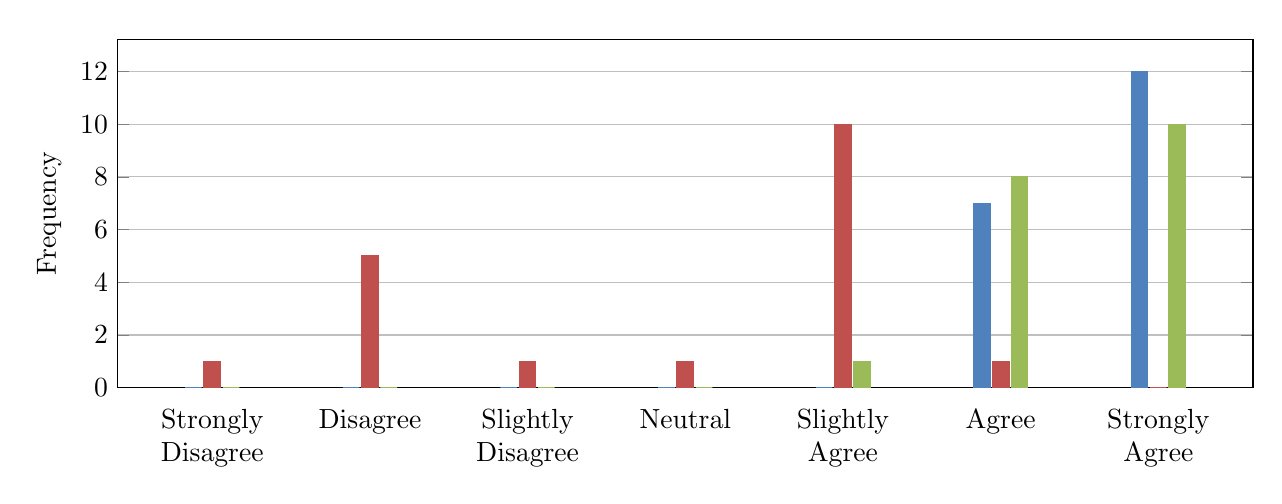
\begin{tikzpicture}
    \begin{axis}[
      width  = 16cm,
      height = 6cm,
      major x tick style = transparent,
      ybar=2*\pgflinewidth,
      bar width=6pt,
      ymajorgrids = true,
      ylabel = {Frequency},
      %xlabel = {Likert Scale Result},
      symbolic x coords= {-3,-2,-1,0,1,2,3},
      xticklabels = {Strongly Disagree,Disagree,Slightly Disagree,Neutral,Slightly Agree,Agree,Strongly Agree},
      xtick = data,
      ytick = {0,2,4,6,8,10,12,14},
      x tick label style  = {text width=2cm,align=center},
      scaled y ticks = false,
      % enlarge x limits=0.25,
      ymin=0,
      legend cell align=left,
      legend style={
              at={(1,1.05)},
              anchor=south east,
              column sep=1ex
      }
    ]
    \addplot[style={bblue,fill=bblue,mark=none}]
    	coordinates {(-3,0) (-2,0) (-1,0) (0,0) (1,0) (2,7) (3,12) };
    \addplot[style={rred,fill=rred,mark=none}]
    	coordinates {(-3,1) (-2,5) (-1,1) (0,1) (1,10) (2,1) (3,0) };
    \addplot[style={ggreen,fill=ggreen,mark=none}]
    	coordinates {(-3,0) (-2,0) (-1,0) (0,0) (1,1) (2,8) (3,10) };

    \end{axis}
\end{tikzpicture}

% \vspace{-20pt}
\paragraph{} Depending on its use, the inferred octave notation makes octaves harder to infer. However, distribution of responses for this question is not significantly different to uniform. Overall this addition was significantly preferable.

\subsection{Nested Instructions}

\begin{table}[!htbp]
\centering
% \caption{Grammar rules for turtle movement instructions. $z \in \mathbb{Z}, n \in \mathbb{N}, c \in \texttt{[A-Za-z]}^{+}$.}
\vspace{1pt}
\begin{tabular}{|l|l|l|} \hline
\textbf{Statement}&\textbf{Mode}&\textbf{p-value}\\ \hline
\mycbox{bblue} It is easier to parse the turtle instruction and tell &Agree&0.0003\\
what it will do.&& \\ \hline
\mycbox{rred} It is easier to repeat sections of notes.&Strongly Agree&0.0000\\ \hline
\mycbox{ggreen} Overall, system 2 is preferable.&Strongly Agree&0.0000\\ \hline
\end{tabular}
\label{evaluation:nestedInstructions}
\end{table}

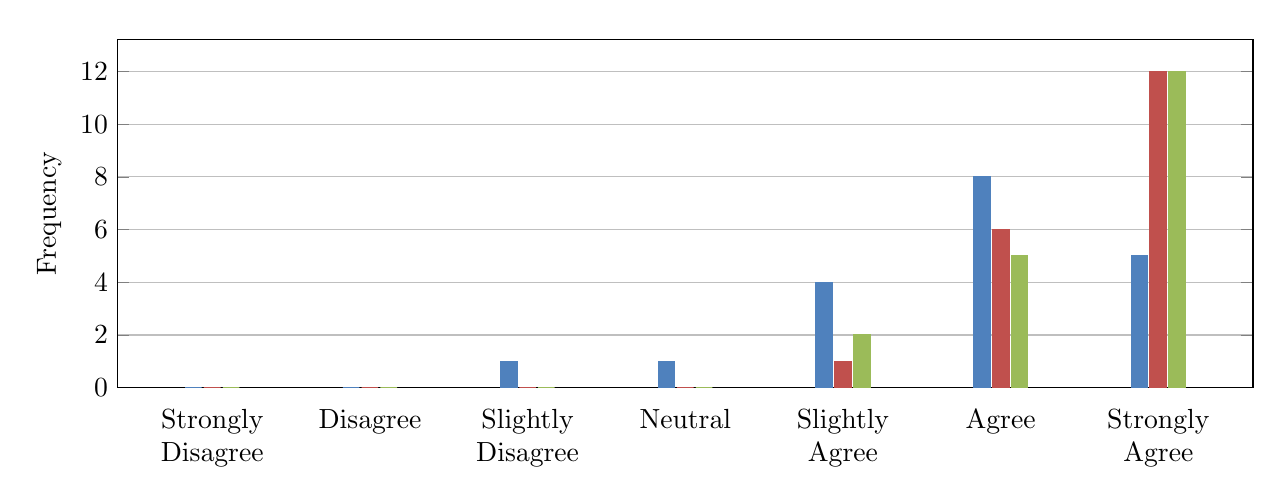
\begin{tikzpicture}
    \begin{axis}[
      % width  = \textwidth,
      width = 16cm,
      height = 6cm,
      major x tick style = transparent,
      ybar=2*\pgflinewidth,
      bar width=6pt,
      ymajorgrids = true,
      ylabel = {Frequency},
      %xlabel = {Likert Scale Result},
      symbolic x coords= {-3,-2,-1,0,1,2,3},
      xticklabels = {Strongly Disagree,Disagree,Slightly Disagree,Neutral,Slightly Agree,Agree,Strongly Agree},
      xtick = data,
      ytick = {0,2,4,6,8,10,12,14},
      x tick label style  = {text width=2cm,align=center},
      scaled y ticks = false,
      % enlarge x limits=0.25,
      ymin=0,
      legend cell align=left,
      legend style={
              at={(1,1.05)},
              anchor=south east,
              column sep=1ex
      }
    ]
    \addplot[style={bblue,fill=bblue,mark=none}]
    coordinates {(-3,0) (-2,0) (-1,1) (0,1) (1,4) (2,8) (3,5) };
    \addplot[style={rred,fill=rred,mark=none}]
    coordinates {(-3,0) (-2,0) (-1,0) (0,0) (1,1) (2,6) (3,12) };
    \addplot[style={ggreen,fill=ggreen,mark=none}]
    coordinates {(-3,0) (-2,0) (-1,0) (0,0) (1,2) (2,5) (3,12) };

        % \legend{It is easier to figure out the turtles path,It is easier to figure out what dynamics different notes are played at,It is easier to tell the order in which dynamics are applied,It is easier to write dynamics in the correct place,Overall system 2 is preferable}
    \end{axis}
\end{tikzpicture}

\paragraph{} All participants found the addition of nested instructions with repeats preferable, with the majority strongly agreeing.

\subsection{Active Turtles List}

\begin{table}[!htbp]
\centering
% \caption{Grammar rules for turtle movement instructions. $z \in \mathbb{Z}, n \in \mathbb{N}, c \in \texttt{[A-Za-z]}^{+}$.}
\vspace{1pt}
\begin{tabular}{|l|l|l|} \hline
\textbf{Statement}&\textbf{Mode}&\textbf{p-value}\\ \hline
\mycbox{bblue} It is easier to tell if a certain turtle has been registered.&Strongly Agree&0.0000\\ \hline
\mycbox{rred} It is easier to see where the active turtles are.&(Strongly) Agree&0.0011\\\hline
\mycbox{ggreen} It is easier to toggle the activation of turtles.&Agree&0.0038 \\ \hline
\mycbox{ppurple} Overall, system 2 is preferable.&Strongly Agree&0.0000 \\ \hline
\end{tabular}
\label{evaluation:activeTurtles}
\end{table}

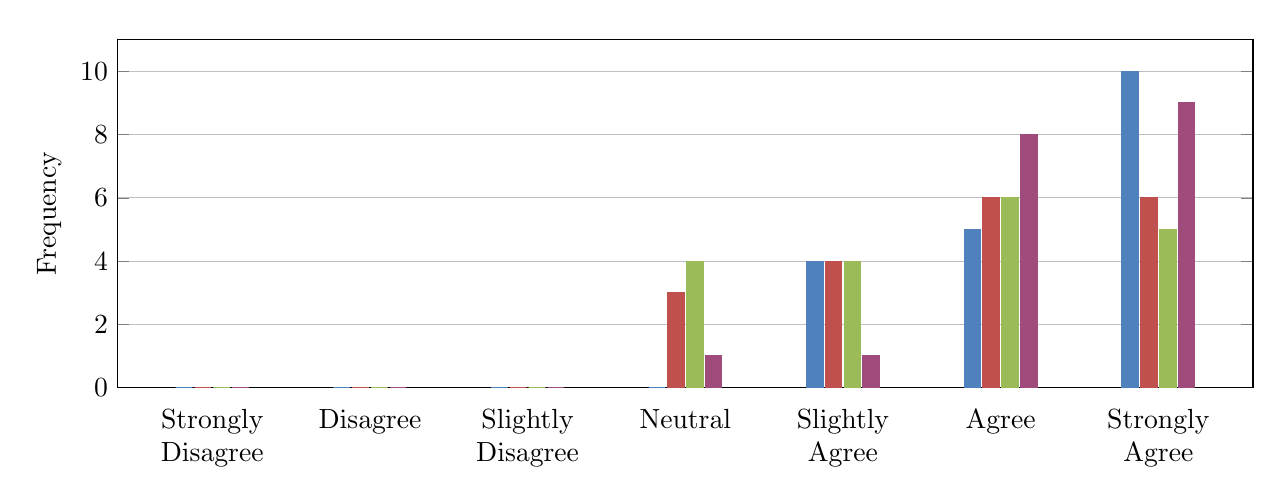
\begin{tikzpicture}
    \begin{axis}[
      % width  = \textwidth,
      width = 16cm,
      height = 6cm,
      major x tick style = transparent,
      ybar=2*\pgflinewidth,
      bar width=6pt,
      ymajorgrids = true,
      ylabel = {Frequency},
      %xlabel = {Likert Scale Result},
      symbolic x coords= {-3,-2,-1,0,1,2,3},
      xticklabels = {Strongly Disagree,Disagree,Slightly Disagree,Neutral,Slightly Agree,Agree,Strongly Agree},
      xtick = data,
      ytick = {0,2,4,6,8,10,12,14},
      x tick label style  = {text width=2cm,align=center},
      scaled y ticks = false,
      % enlarge x limits=0.25,
      ymin=0,
      legend cell align=left,
      legend style={
              at={(1,1.05)},
              anchor=south east,
              column sep=1ex
      }
    ]
    \addplot[style={bblue,fill=bblue,mark=none}]
    coordinates {(-3,0) (-2,0) (-1,0) (0,0) (1,4) (2,5) (3,10) };
    \addplot[style={rred,fill=rred,mark=none}]
    coordinates {(-3,0) (-2,0) (-1,0) (0,3) (1,4) (2,6) (3,6) };
    \addplot[style={ggreen,fill=ggreen,mark=none}]
    coordinates {(-3,0) (-2,0) (-1,0) (0,4) (1,4) (2,6) (3,5) };
    \addplot[style={ppurple,fill=ppurple,mark=none}]
    coordinates {(-3,0) (-2,0) (-1,0) (0,1) (1,1) (2,8) (3,9) };

        % \legend{It is easier to figure out the turtles path,It is easier to figure out what dynamics different notes are played at,It is easier to tell the order in which dynamics are applied,It is easier to write dynamics in the correct place,Overall system 2 is preferable}
    \end{axis}
\end{tikzpicture}

\paragraph{} The addition of a list of active turtles was found by all users to have a neutral or possitive effect on Excello.

\subsection{Continuous Volume}

\begin{table}[!htbp]
\centering
% \caption{Grammar rules for turtle movement instructions. $z \in \mathbb{Z}, n \in \mathbb{N}, c \in \texttt{[A-Za-z]}^{+}$.}
\vspace{1pt}
\begin{tabular}{|l|l|l|} \hline
\textbf{Statement}&\textbf{Mode}&\textbf{p-value}\\ \hline
\mycbox{bblue} It is more intuitive how loud a note will be played.&Disagree&0.6592\\
&Strongly Agree& \\ \hline
\mycbox{rred} The volumes available are less limited.&Strongly Agree&0.0000\\ \hline
\mycbox{ggreen} Overall, system 2 is preferable..&Agree&0.0003\\ \hline
\end{tabular}
\label{evaluation:continuousVolume}
\end{table}

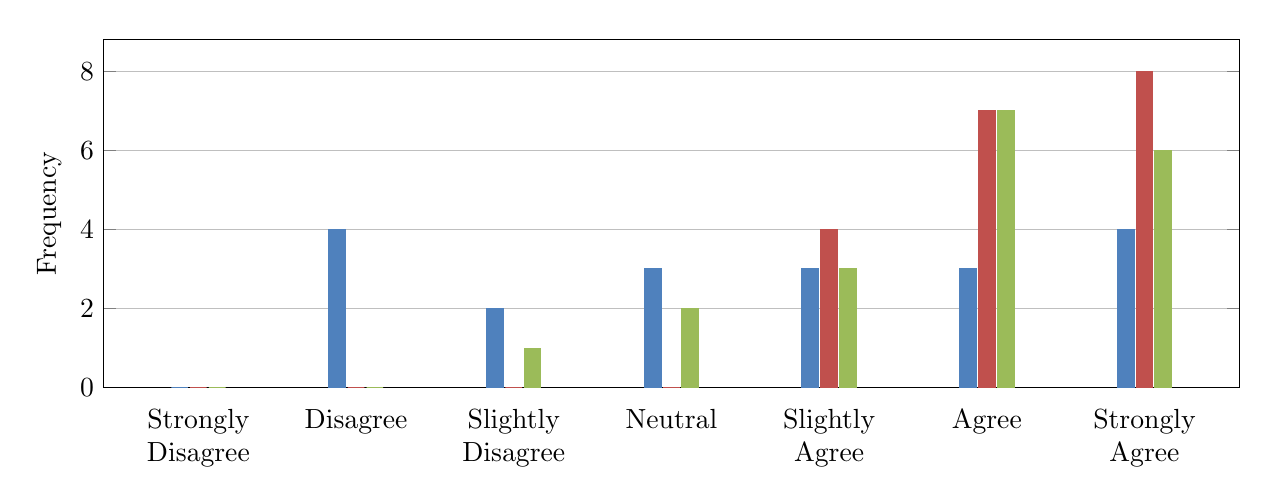
\begin{tikzpicture}
    \begin{axis}[
      % width  = \textwidth,
      width = 16cm,
      height = 6cm,
      major x tick style = transparent,
      ybar=2*\pgflinewidth,
      bar width=6pt,
      ymajorgrids = true,
      ylabel = {Frequency},
      %xlabel = {Likert Scale Result},
      symbolic x coords= {-3,-2,-1,0,1,2,3},
      xticklabels = {Strongly Disagree,Disagree,Slightly Disagree,Neutral,Slightly Agree,Agree,Strongly Agree},
      xtick = data,
      ytick = {0,2,4,6,8,10,12,14},
      x tick label style  = {text width=2cm,align=center},
      scaled y ticks = false,
      % enlarge x limits=0.25,
      ymin=0,
      legend cell align=left,
      legend style={
              at={(1,1.05)},
              anchor=south east,
              column sep=1ex
      }
    ]
    \addplot[style={bblue,fill=bblue,mark=none}]
    coordinates {(-3,0) (-2,4) (-1,2) (0,3) (1,3) (2,3) (3,4) };
    \addplot[style={rred,fill=rred,mark=none}]
    coordinates {(-3,0) (-2,0) (-1,0) (0,0) (1,4) (2,7) (3,8) };
    \addplot[style={ggreen,fill=ggreen,mark=none}]
    coordinates {(-3,0) (-2,0) (-1,1) (0,2) (1,3) (2,7) (3,6) };

        % \legend{It is easier to figure out the turtles path,It is easier to figure out what dynamics different notes are played at,It is easier to tell the order in which dynamics are applied,It is easier to write dynamics in the correct place,Overall system 2 is preferable}
    \end{axis}
\end{tikzpicture}

\paragraph{} There is no significant result for whether the ability to define volume in the range [0,1] is more intuitive. All users agreed that the volumes were less confined. However, only one user did not find this change preferable. Given that, it can be ommitted and the previous conventional dynamic markings used, this supports the addition being successful.

\subsection{Automatic Stepping}

\begin{table}[!htbp]
\centering
% \caption{Grammar rules for turtle movement instructions. $z \in \mathbb{Z}, n \in \mathbb{N}, c \in \texttt{[A-Za-z]}^{+}$.}
\vspace{1pt}
\begin{tabular}{|l|l|l|} \hline
\textbf{Statement}&\textbf{Mode}&\textbf{p-value}\\ \hline
\mycbox{bblue} Less mental work is required to write the turtle. &Strongly Agree&0.0000\\
instructions.&& \\ \hline
\mycbox{rred} Less work is required when more notes wish to be added.&Strongly Agree&0.0000\\ \hline
\mycbox{ggreen} Overall, system 2 is preferable.&Strongly Agree&0.0000\\ \hline
\end{tabular}
\label{evaluation:automaticStepping}
\end{table}

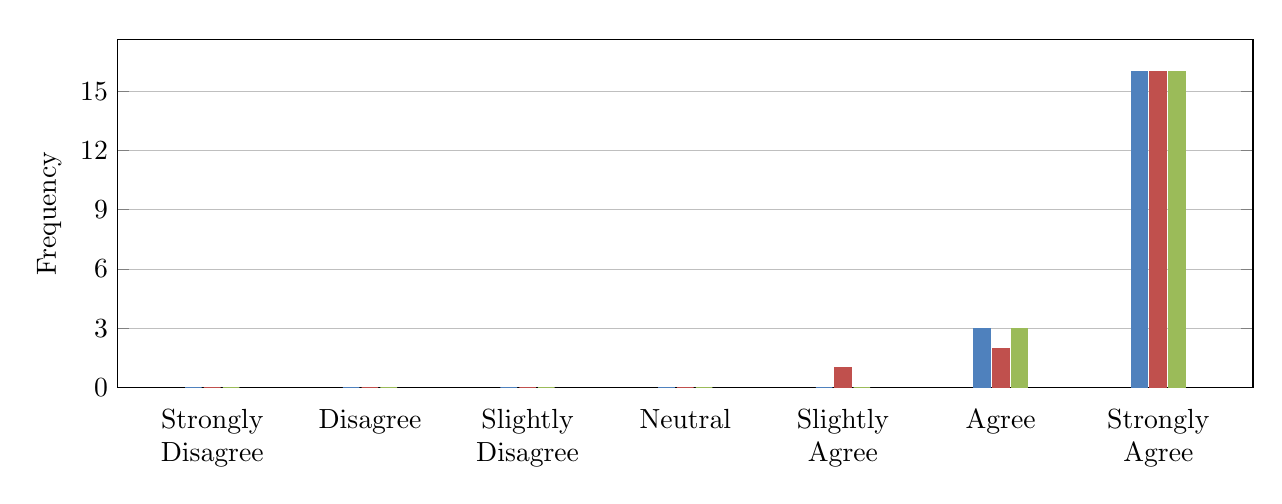
\begin{tikzpicture}
    \begin{axis}[
      % width  = \textwidth,
      width = 16cm,
      height = 6cm,
      major x tick style = transparent,
      ybar=2*\pgflinewidth,
      bar width=6pt,
      ymajorgrids = true,
      ylabel = {Frequency},
      %xlabel = {Likert Scale Result},
      symbolic x coords= {-3,-2,-1,0,1,2,3},
      xticklabels = {Strongly Disagree,Disagree,Slightly Disagree,Neutral,Slightly Agree,Agree,Strongly Agree},
      xtick = data,
      ytick = {0,3,6,9,12,15},
      x tick label style  = {text width=2cm,align=center},
      scaled y ticks = false,
      % enlarge x limits=0.25,
      ymin=0,
      legend cell align=left,
      legend style={
              at={(1,1.05)},
              anchor=south east,
              column sep=1ex
      }
    ]
    \addplot[style={bblue,fill=bblue,mark=none}]
    coordinates {(-3,0) (-2,0) (-1,0) (0,0) (1,0) (2,3) (3,16) };
    \addplot[style={rred,fill=rred,mark=none}]
    coordinates {(-3,0) (-2,0) (-1,0) (0,0) (1,1) (2,2) (3,16) };
    \addplot[style={ggreen,fill=ggreen,mark=none}]
    coordinates {(-3,0) (-2,0) (-1,0) (0,0) (1,0) (2,3) (3,16) };

        % \legend{It is easier to figure out the turtles path,It is easier to figure out what dynamics different notes are played at,It is easier to tell the order in which dynamics are applied,It is easier to write dynamics in the correct place,Overall system 2 is preferable}
    \end{axis}
\end{tikzpicture}

\paragraph{} The addition of this feature was particularly successful with 16 of the 19 users strongly agreeing the system was more preferable with automatic stepping available in the turtle instructions.

\subsection{Absolute Tempo}

\begin{table}[!htbp]
\centering
% \caption{Grammar rules for turtle movement instructions. $z \in \mathbb{Z}, n \in \mathbb{N}, c \in \texttt{[A-Za-z]}^{+}$.}
\vspace{1pt}
\begin{tabular}{|l|l|l|} \hline
\textbf{Statement}&\textbf{Mode}&\textbf{p-value}\\ \hline
\mycbox{bblue} It is easier to tell what the speed instruction&Strongly Agree&0.0000\\
 corresponds to.&& \\ \hline
\mycbox{rred} Giving an exact tempo (e.g. when transcribing sheet&Strongly Agree&0.0000\\
music) is easier.&& \\ \hline
\mycbox{ggreen} Overall, system 2 is preferable.&Strongly Agree&0.0000\\ \hline
\end{tabular}
\label{evaluation:absoluteTempo}
\end{table}

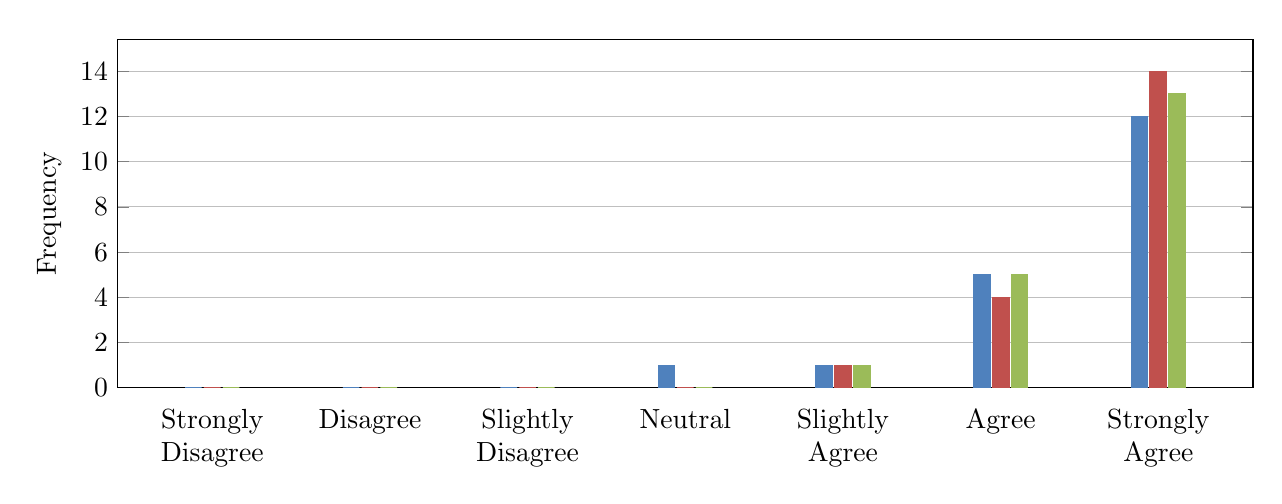
\begin{tikzpicture}
    \begin{axis}[
      % width  = \textwidth,
      width = 16cm,
      height = 6cm,
      major x tick style = transparent,
      ybar=2*\pgflinewidth,
      bar width=6pt,
      ymajorgrids = true,
      ylabel = {Frequency},
      %xlabel = {Likert Scale Result},
      symbolic x coords= {-3,-2,-1,0,1,2,3},
      xticklabels = {Strongly Disagree,Disagree,Slightly Disagree,Neutral,Slightly Agree,Agree,Strongly Agree},
      xtick = data,
      ytick = {0,2,4,6,8,10,12,14},
      x tick label style  = {text width=2cm,align=center},
      scaled y ticks = false,
      % enlarge x limits=0.25,
      ymin=0,
      legend cell align=left,
      legend style={
              at={(1,1.05)},
              anchor=south east,
              column sep=1ex
      }
    ]
    \addplot[style={bblue,fill=bblue,mark=none}]
    coordinates {(-3,0) (-2,0) (-1,0) (0,1) (1,1) (2,5) (3,12) };
    \addplot[style={rred,fill=rred,mark=none}]
    coordinates {(-3,0) (-2,0) (-1,0) (0,0) (1,1) (2,4) (3,14) };
    \addplot[style={ggreen,fill=ggreen,mark=none}]
    coordinates {(-3,0) (-2,0) (-1,0) (0,0) (1,1) (2,5) (3,13) };

        % \legend{It is easier to figure out the turtles path,It is easier to figure out what dynamics different notes are played at,It is easier to tell the order in which dynamics are applied,It is easier to write dynamics in the correct place,Overall system 2 is preferable}
    \end{axis}
\end{tikzpicture}

\paragraph{} The initial design was changed so that turtle speed was defined in absolute cells per minute. All users found this to be an improvement.

\paragraph{} Overall, the participatory design process was very successful. Multiple features were added to Excello to solve problems identified through formative evaluation sessions and longer-term feedback from users. There is signficant evidence to suggest all added features were found to improve Excello.

\section{Cognitive Dimensions of Notation}

\paragraph{} Figure \ref{fig:usage} shows the time users identified carrying out the different cognitive activities \cite{blackwell:tutorial} in Excello and in Sibelius. There are 19 users for Excello and 12 for Sibelius. This shows Translation is a very important activity for both interfaces. There is more exploratory design for Excello but as users become more familiar with the system and the amount of existing Excello notation increases, modification and incrementation may become more important. Little time is spent searching for information in the notaiton in either.

\begin{figure}[ht]
\centering
\begin{subfigure}{.6\textwidth}
  \centering
    \begin{tikzpicture}
      \begin{axis}
        [
        height = 8cm,
        width = 7cm,
        ytick={1,2,3,4,5},
        yticklabels={Searching, Translation, Incrementation, Modification, Exploratory Design},
        xlabel = {Percentage of Time}
        ]
        \addplot+[
        	boxplot prepared={
        		median=10,
        		upper quartile=3.319672131,
        		lower quartile=10,
        		upper whisker=30,
        		lower whisker=0
        	},
        ] coordinates {};
        \addplot+[
        	boxplot prepared={
        		median=50,
        		upper quartile=45,
        		lower quartile=65,
        		upper whisker=100,
        		lower whisker=8
        	},
        ] coordinates {};
        \addplot+[
        	boxplot prepared={
        		median=10,
        		upper quartile=5,
        		lower quartile=15.69672131,
        		upper whisker=24,
        		lower whisker=0
        	},
        ] coordinates {};
        \addplot+[
        	boxplot prepared={
        		median=10,
        		upper quartile=5,
        		lower quartile=15.69672131,
        		upper whisker=30,
        		lower whisker=0
        	},
        ] coordinates {};
        \addplot+[
        	boxplot prepared={
        		median=10,
        		upper quartile=9,
        		lower quartile=27,
        		upper whisker=49,
        		lower whisker=0
        	},
        ] coordinates {};
      \end{axis}
    \end{tikzpicture}
  % \caption{A subfigure}
  \label{fig:sub1}
\end{subfigure}%
\begin{subfigure}{.4\textwidth}
  \centering
    \begin{tikzpicture}
      \begin{axis}
        [
        height = 8cm,
        width = 6.5cm,
        ytick={1,2,3,4,5},
        yticklabels={},
        xlabel = {Percentage of Time}
        ]
        \addplot+[
          boxplot prepared={
            median=10,
            upper quartile=5,
            lower quartile=11,
            upper whisker=27.27272727,
            lower whisker=0.460829493
          },
        ] coordinates {};
        \addplot+[
          boxplot prepared={
            median=40.22727273,
            upper quartile=30,
            lower quartile=50,
            upper whisker=60,
            lower whisker=13.82488479
          },
        ] coordinates {};
        \addplot+[
          boxplot prepared={
            median=20,
            upper quartile=15,
            lower quartile=29.25,
            upper whisker=41.47465438,
            lower whisker=4.545454545
          },
        ] coordinates {};
        \addplot+[
          boxplot prepared={
            median=16.09090909,
            upper quartile=10,
            lower quartile=30,
            upper whisker=41.47465438,
            lower whisker=5
          },
        ] coordinates {};
        \addplot+[
          boxplot prepared={
            median=9.166666667,
            upper quartile=4.886363636,
            lower quartile=15,
            upper whisker=20,
            lower whisker=0
          },
        ] coordinates {};
      \end{axis}
    \end{tikzpicture}
  % \caption{A subfigure}
  \label{fig:sub2}
\end{subfigure}
\caption{The percentage of time spent performing the different cognitive activites in Excello (left) and Sibelius (right).}
\label{fig:usage}
\end{figure}

\paragraph{} A series of statements from \cite{blackwell:questionnaire} were selected to assess the CDN of Excello. Users responded with a five-point (Strongly Disagree, Disagree, Neutral, Agree, Strongly Agree) Likert scale. The significance of the results was verified with a chi-squared test. First the data was combined into negative and non-negative categories. The dimension being assessed, p-value from the chi-squared test and modal repsonse for each statement are shown in table \ref{evaluation:cdnTable}. The distribution of responses is shown in figure \ref{evaluation:cdnQuestions}.

\begin{table}[!htbp]
\centering
\vspace{1pt}
\begin{tabular}{|l|l|l|l|} \hline
\textbf{Statement}&\textbf{CDN}&\textbf{Mode}&\textbf{p-value}\\ \hline
\mycbox{bblue} (a) The notation used (In Excello: notes/ &Closeness&Agree&0.0004\\
dynamics in cells and the definition of turtles)&of&& \\
is related to the result you are describing (In &Mapping&& \\
Excello: Musical output)&&& \\ \hline
\mycbox{rred} (b) Where there are different parts of the&Consistency&Agree&0.0087\\
notation that mean similar things, the&&& \\
similarity is clear from the way they appear. &&& \\ \hline
\mycbox{ggreen} (c) You can add extra marks (or colours or &Secondary&Agree&0.0020\\
format choices) to clarify, emphasise or repeat&Notation&& \\
what is there already. &&& \\ \hline
\mycbox{ppurple} (d) When you need to make changes to&Viscosity&Agree&0.0004 \\
previous, work it is easy to make the change.&&& \\ \hline
\mycbox{yyellow} (e) It is easy to see or find the various parts of &Visibility/&Agree&0.0087 \\
the notation while it is being created or changed.&Juxtaposition&& \\ \hline
\mycbox{bbrown} (f) If you need to compare or combine different&Visibility/&Agree&0.0312 \\
parts, you cansee them at the same time.&Juxtaposition&& \\ \hline
\end{tabular}
\caption{Questions and results for testing the CDN of Excello \label{evaluation:cdnTable}}
\end{table}

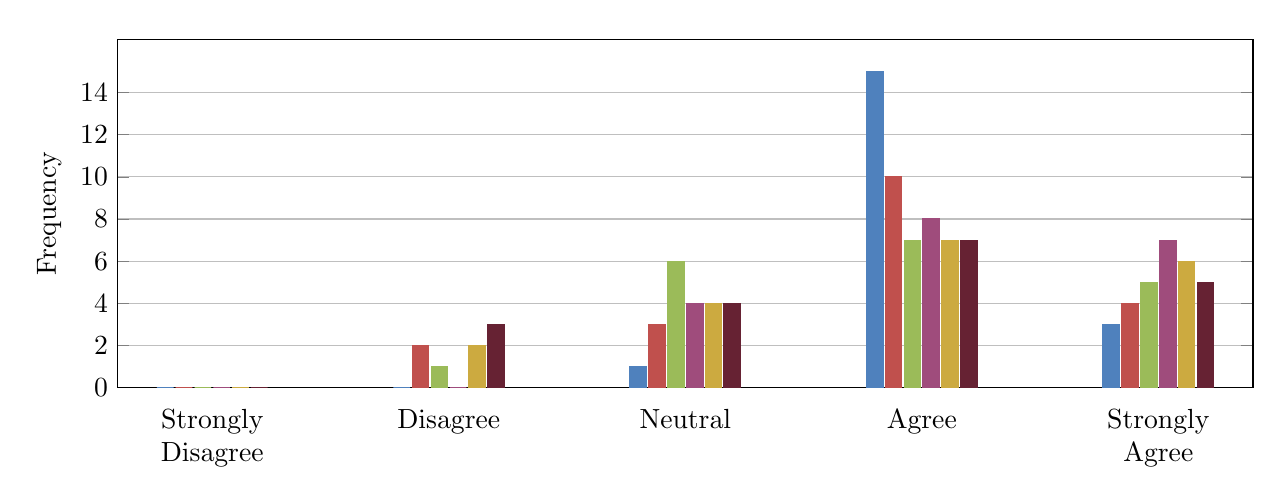
\begin{tikzpicture}
    \begin{axis}[
      % width  = \textwidth,
      width = 16cm,
      height = 6cm,
      major x tick style = transparent,
      ybar=2*\pgflinewidth,
      bar width=6pt,
      ymajorgrids = true,
      ylabel = {Frequency},
      %xlabel = {Likert Scale Result},
      symbolic x coords= {-3,-2,-1,0,1,2,3},
      xticklabels = {Strongly Disagree,Disagree,Neutral,Agree,Strongly Agree},
      xtick = data,
      ytick = {0,2,4,6,8,10,12,14},
      x tick label style  = {text width=2cm,align=center},
      scaled y ticks = false,
      % enlarge x limits=0.25,
      ymin=0,
      legend cell align=left,
      legend style={
              at={(1,1.05)},
              anchor=south east,
              column sep=1ex
      }
    ]
    \addplot[style={bblue,fill=bblue,mark=none}]
    	coordinates {(-3,0) (-2,0) (-1,1) (0,15) (1,3) };
    \addplot[style={rred,fill=rred,mark=none}]
    	coordinates {(-3,0) (-2,2) (-1,3) (0,10) (1,4) };
    \addplot[style={ggreen,fill=ggreen,mark=none}]
    	coordinates {(-3,0) (-2,1) (-1,6) (0,7) (1,5) };
    \addplot[style={ppurple,fill=ppurple,mark=none}]
    	coordinates {(-3,0) (-2,0) (-1,4) (0,8) (1,7) };
    \addplot[style={yyellow,fill=yyellow,mark=none}]
    	coordinates {(-3,0) (-2,2) (-1,4) (0,7) (1,6) };
    \addplot[style={bbrown,fill=bbrown,mark=none}]
    	coordinates {(-3,0) (-2,3) (-1,4) (0,7) (1,5) };

    \end{axis}
\end{tikzpicture}
\label{evaluation:cdnQuestions}

\paragraph{} As these questions were also answered for the user's interface of choice, a comparison to Sibelius is made. As the data does not meet the assumptions of the t-test \cite{barry:likert}, I perofrmed a Wilcoxon matchd pairs signed-ranked test on the 12 pairs by encoding the five possible responses as -2,-1,0,1,2. For all six questions, there is no indication that the answers for the two interfaces come from populations with different means.

\subsection{Closeness of Mapping}

\paragraph{} As there is no significant evidence that the population means for Excello and Sibelius were different, this suggests Excello's notation with spreadsheets has not compromised that closeness of mapping of traditional notation. This is helped by using an existing notation (SPN) for defining the individual notes, the turtle instructions mapping to a movement through the grid, and by adjusting the speed argument to be an absolute, not relative, parameter. Being less familiar with staff notation, user 4 found Sibelius's notation unintuitive.

\begin{figure}[htb]
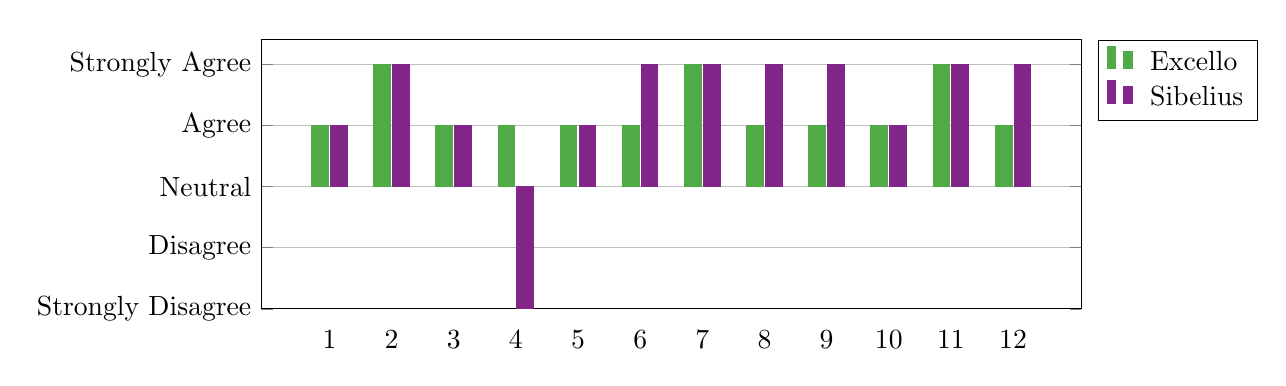
\begin{tikzpicture}
    \begin{axis}[
      % width  = \textwidth,
      width = 12cm,
      height = 5cm,
      major x tick style = transparent,
      ybar=2*\pgflinewidth,
      bar width=6pt,
      ymajorgrids = true,
      % ylabel = {Frequency},
      % %xlabel = {Likert Scale Result},
      % symbolic y coords= {-2,-1,0,1,2},
      yticklabels = {Strongly Disagree,Disagree,Neutral,Agree,Strongly Agree},
      xtick = {1,2,3,4,5,6,7,8,9,10,11,12},
      ytick = {-2,-1,0,1,2},
      ymin = -2,
      x tick label style  = {text width=2cm,align=center},
      scaled y ticks = false,
      % enlarge x limits=0.25,
      legend cell align=left,
      legend style={
              at={(1.02,1)},
              anchor=north west,
              column sep=1ex
      }
    ]
    \addplot[style={excelGreen,fill=excelGreen,mark=none}]
    	coordinates {(1,1) (2,2) (3,1) (4,1) (5,1) (6,1) (7,2) (8,1) (9,1) (10,1) (11,2) (12,1) };
    \addplot[style={sibPurple,fill=sibPurple,mark=none}]
    	coordinates {(1,1) (2,2) (3,1) (4,-2) (5,1) (6,2) (7,2) (8,2) (9,2) (10,1) (11,2) (12,2) };

    \legend{Excello,Sibelius}

    \end{axis}
\end{tikzpicture}
\caption{User responses for \textit{closeness of mapping} for Excello and Sibelius from (a)}
\label{evaluation:clos}
\end{figure}

\subsection{Consistency}

\paragraph{} As each cell and turtle only causes one note to play at a time, consistency is maintained by building pieces from these elements. Excello keeps consistency with Excel by sharing notations (e.g. A1:A5 for ranges) and using the existing formula editor. Within the turtle instructions, using a number after instructions to repeat holds for both individual instructions and sequences. This all contributes to no significant result from the Wilcoxon test.

\begin{figure}[htb]
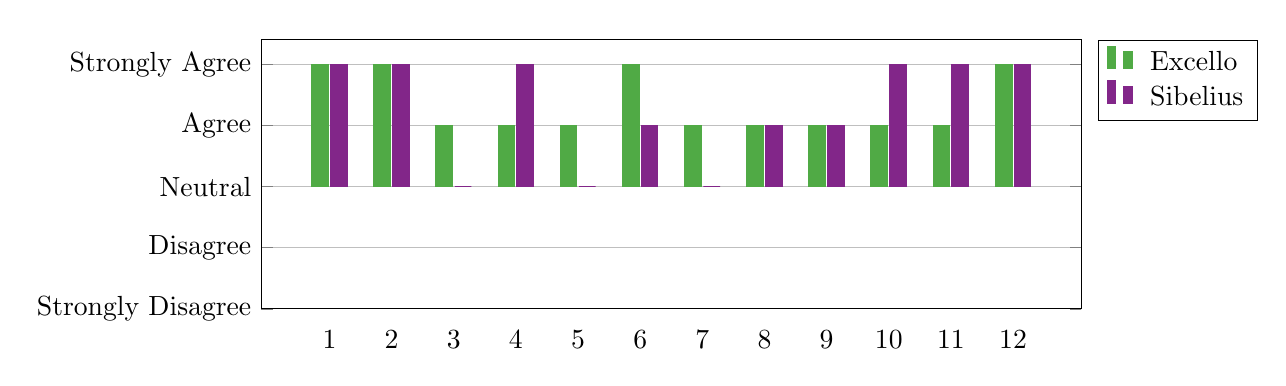
\begin{tikzpicture}
    \begin{axis}[
      % width  = \textwidth,
      width = 12cm,
      height = 5cm,
      major x tick style = transparent,
      ybar=2*\pgflinewidth,
      bar width=6pt,
      ymajorgrids = true,
      % ylabel = {Frequency},
      % %xlabel = {Likert Scale Result},
      % symbolic y coords= {-2,-1,0,1,2},
      yticklabels = {Strongly Disagree,Disagree,Neutral,Agree,Strongly Agree},
      xtick = {1,2,3,4,5,6,7,8,9,10,11,12},
      ytick = {-2,-1,0,1,2},
      ymin = -2,
      x tick label style  = {text width=2cm,align=center},
      scaled y ticks = false,
      % enlarge x limits=0.25,
      legend cell align=left,
      legend style={
              at={(1.02,1)},
              anchor=north west,
              column sep=1ex
      }
    ]

    \addplot[style={excelGreen,fill=excelGreen,mark=none}]
    	coordinates {(1,2) (2,2) (3,1) (4,1) (5,1) (6,2) (7,1) (8,1) (9,1) (10,1) (11,1) (12,2) };
    \addplot[style={sibPurple,fill=sibPurple,mark=none}]
    	coordinates {(1,2) (2,2) (3,0) (4,2) (5,0) (6,1) (7,0) (8,1) (9,1) (10,2) (11,2) (12,2) };

    \legend{Excello,Sibelius}

    \end{axis}
\end{tikzpicture}
\caption{User responses for \textit{consistency} for Excello and Sibelius from (b)}
\label{evaluation:cons}
\end{figure}

\subsection{Secondary Notation}

\paragraph{} Given the translation time, secondary notation is particularly important \cite{blackwell:notation}. Given that Excello abstracts time from the axes of the grid the distribution of parts is up to the user and cells can be used for arbitrary marks. Therefore, existing Excel features for formatting and grouping cells remain available. This is utilised by the automatic highlighting of notes and turtles. That there is no significant difference in population means, this suggests that the spreadsheet paradigm can provide equal secondary notaion abilities to Sibelius, software already equipped with numerous ways to customise a score.

\begin{figure}[tbh]
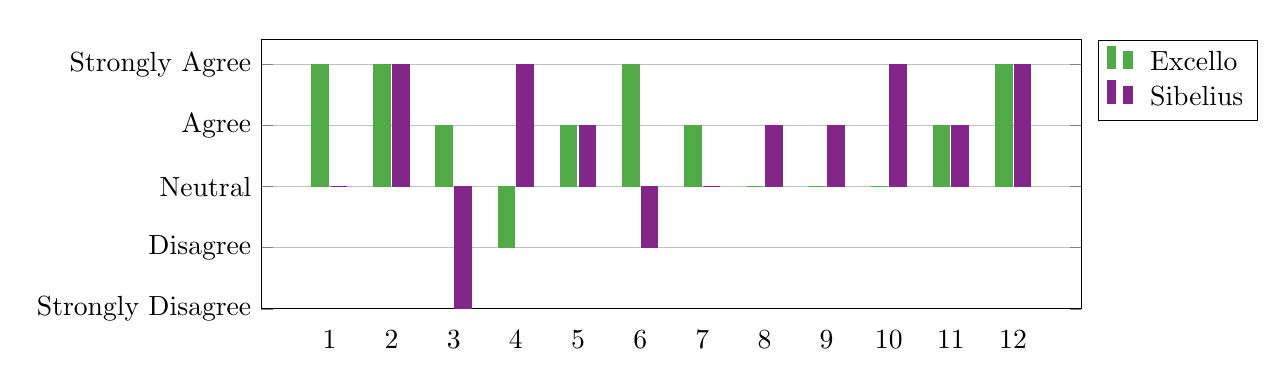
\begin{tikzpicture}
    \begin{axis}[
      % width  = \textwidth,
      width = 12cm,
      height = 5cm,
      major x tick style = transparent,
      ybar=2*\pgflinewidth,
      bar width=6pt,
      ymajorgrids = true,
      % ylabel = {Frequency},
      % %xlabel = {Likert Scale Result},
      % symbolic y coords= {-2,-1,0,1,2},
      yticklabels = {Strongly Disagree,Disagree,Neutral,Agree,Strongly Agree},
      xtick = {1,2,3,4,5,6,7,8,9,10,11,12},
      ytick = {-2,-1,0,1,2},
      ymin = -2,
      x tick label style  = {text width=2cm,align=center},
      scaled y ticks = false,
      % enlarge x limits=0.25,
      legend cell align=left,
      legend style={
              at={(1.02,1)},
              anchor=north west,
              column sep=1ex
      }
    ]

    \addplot[style={excelGreen,fill=excelGreen,mark=none}]
      coordinates {(1,2) (2,2) (3,1) (4,-1) (5,1) (6,2) (7,1) (8,0) (9,0) (10,0) (11,1) (12,2) };
    \addplot[style={sibPurple,fill=sibPurple,mark=none}]
      coordinates {(1,0) (2,2) (3,-2) (4,2) (5,1) (6,-1) (7,0) (8,1) (9,1) (10,2) (11,1) (12,2) };

    \legend{Excello,Sibelius}

    \end{axis}
\end{tikzpicture}
\caption{User responses for \textit{secondary notation} for Excello and Sibelius from (c)}
\label{evaluation:secn}
\end{figure}

\subsection{Viscosity}

\paragraph{} By allowing dynamics and octave marking to be ommitted and the ability for turtles to step forward automatically, there is low resistance to making additions and changes to the music. The toggling of turtle activations dramatically reduces the actions required to turn turtles on and off. Furthermore Excel allows for the easy editing and movement of cells. No significant result in the Wilcoxon test suggests the interfaces have comparable viscosity.

\begin{figure}[tbh]
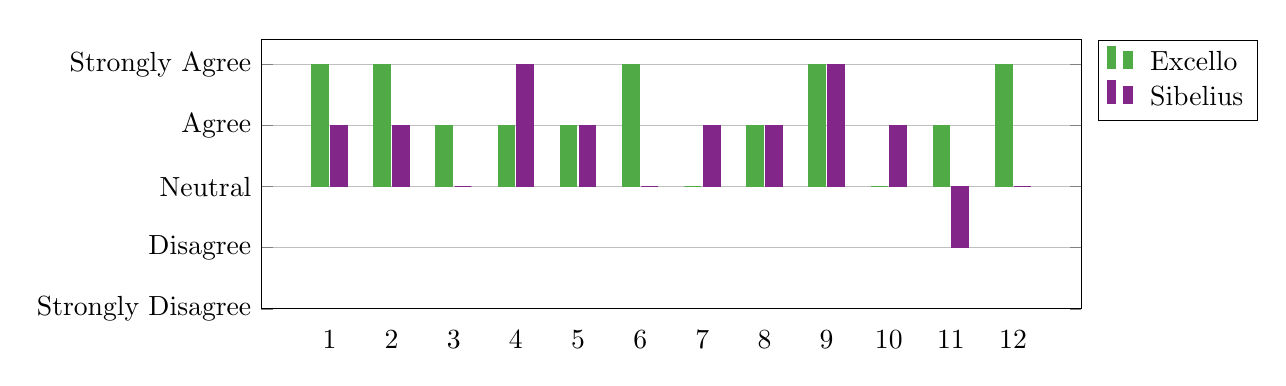
\begin{tikzpicture}
    \begin{axis}[
      % width  = \textwidth,
      width = 12cm,
      height = 5cm,
      major x tick style = transparent,
      ybar=2*\pgflinewidth,
      bar width=6pt,
      ymajorgrids = true,
      % ylabel = {Frequency},
      % %xlabel = {Likert Scale Result},
      % symbolic y coords= {-2,-1,0,1,2},
      yticklabels = {Strongly Disagree,Disagree,Neutral,Agree,Strongly Agree},
      xtick = {1,2,3,4,5,6,7,8,9,10,11,12},
      ytick = {-2,-1,0,1,2},
      ymin = -2,
      x tick label style  = {text width=2cm,align=center},
      scaled y ticks = false,
      % enlarge x limits=0.25,
      legend cell align=left,
      legend style={
              at={(1.02,1)},
              anchor=north west,
              column sep=1ex
      }
    ]

    \addplot[style={excelGreen,fill=excelGreen,mark=none}]
    	coordinates {(1,2) (2,2) (3,1) (4,1) (5,1) (6,2) (7,0) (8,1) (9,2) (10,0) (11,1) (12,2) };
    \addplot[style={sibPurple,fill=sibPurple,mark=none}]
    	coordinates {(1,1) (2,1) (3,0) (4,2) (5,1) (6,0) (7,1) (8,1) (9,2) (10,1) (11,-1) (12,0) };

    \legend{Excello,Sibelius}

    \end{axis}
\end{tikzpicture}
\caption{User responses for \textit{viscosity} for Excello and Sibelius from (d)}
\label{evaluation:visc}
\end{figure}

\subsection{Visability / Juxtaposition}

\paragraph{} For both questions there was no significant difference in population mean. This suggests that the speadsheet interface can provide a similar abilty to view components than Sibelius.

\begin{figure}[tbh]
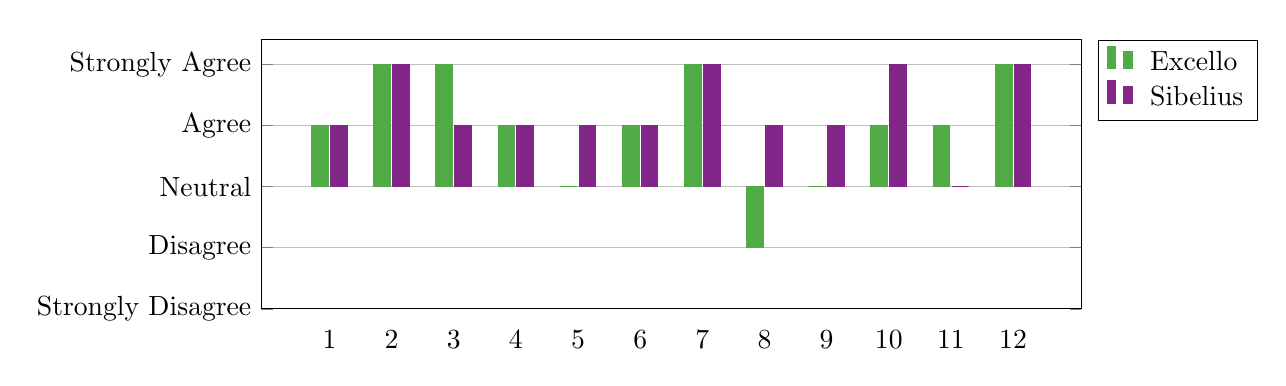
\begin{tikzpicture}
    \begin{axis}[
      % width  = \textwidth,
      width = 12cm,
      height = 5cm,
      major x tick style = transparent,
      ybar=2*\pgflinewidth,
      bar width=6pt,
      ymajorgrids = true,
      % ylabel = {Frequency},
      % %xlabel = {Likert Scale Result},
      % symbolic y coords= {-2,-1,0,1,2},
      yticklabels = {Strongly Disagree,Disagree,Neutral,Agree,Strongly Agree},
      xtick = {1,2,3,4,5,6,7,8,9,10,11,12},
      ytick = {-2,-1,0,1,2},
      ymin = -2,
      x tick label style  = {text width=2cm,align=center},
      scaled y ticks = false,
      % enlarge x limits=0.25,
      legend cell align=left,
      legend style={
              at={(1.02,1)},
              anchor=north west,
              column sep=1ex
      }
    ]

    \addplot[style={excelGreen,fill=excelGreen,mark=none}]
    	coordinates {(1,1) (2,2) (3,2) (4,1) (5,0) (6,1) (7,2) (8,-1) (9,0) (10,1) (11,1) (12,2) };
    \addplot[style={sibPurple,fill=sibPurple,mark=none}]
    	coordinates {(1,1) (2,2) (3,1) (4,1) (5,1) (6,1) (7,2) (8,1) (9,1) (10,2) (11,0) (12,2) };

    \legend{Excello,Sibelius}

    \end{axis}
\end{tikzpicture}
\caption{User responses for \textit{visibility/juxtaposition} for Excello and Sibelius from (e)}
\label{evaluation:viju1}
\end{figure}

\begin{figure}[tbh]
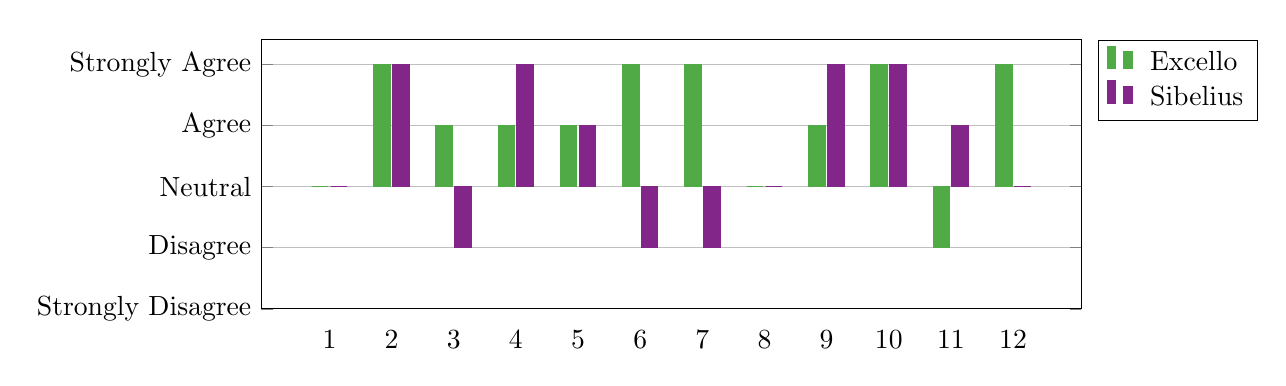
\begin{tikzpicture}
    \begin{axis}[
      % width  = \textwidth,
      width = 12cm,
      height = 5cm,
      major x tick style = transparent,
      ybar=2*\pgflinewidth,
      bar width=6pt,
      ymajorgrids = true,
      % ylabel = {Frequency},
      % %xlabel = {Likert Scale Result},
      % symbolic y coords= {-2,-1,0,1,2},
      yticklabels = {Strongly Disagree,Disagree,Neutral,Agree,Strongly Agree},
      xtick = {1,2,3,4,5,6,7,8,9,10,11,12},
      ytick = {-2,-1,0,1,2},
      ymin = -2,
      x tick label style  = {text width=2cm,align=center},
      scaled y ticks = false,
      % enlarge x limits=0.25,
      legend cell align=left,
      legend style={
              at={(1.02,1)},
              anchor=north west,
              column sep=1ex
      }
    ]

    \addplot[style={excelGreen,fill=excelGreen,mark=none}]
    	coordinates {(1,0) (2,2) (3,1) (4,1) (5,1) (6,2) (7,2) (8,0) (9,1) (10,2) (11,-1) (12,2) };
    \addplot[style={sibPurple,fill=sibPurple,mark=none}]
    	coordinates {(1,0) (2,2) (3,-1) (4,2) (5,1) (6,-1) (7,-1) (8,0) (9,2) (10,2) (11,1) (12,0) };

    \legend{Excello,Sibelius}

    \end{axis}
\end{tikzpicture}
\caption{User responses for \textit{visibility/juxtaposition} for Excello and Sibelius from (f)}
\label{evaluation:viju2}
\end{figure}

\paragraph{} Sibelius uses established music notation as part of large professional software. However, there was no significant evidence to suggest Sibelius outperformed Excello across these CDN. This suggests that despite being built for a genereal purpose spreadsheet environment, Excello is successful interface for writing music.

\subsection{Other Dimensions}

\paragraph{} If users are unfamiliar with the turtle paradigm, this may reduce the \textit{role-expressiveness}. Turtles and notes are the only musical spreadsheet components and are identified by highlighting. Whilst notes and turtles can be added in any order, adding an additional part may require many line insertions which would increase the \textit{premature committment}. The dual-formalism of the turtles and notes could create high \textit{diffuseness} but the user's freedom to lay these out allows this to be minimized as in figure \ref{evaluation:excelloFranzRedacted}. This also shows how representations can have strong \textit{synopsie}, as the notes or turtles don't need to be examined to understand what is happening. This may come at the expense of \textit{hidden dependencies} if it is not immediately clear which notes are triggered by which turtles. Volume is also dependent on the notes turtles play before it. But as a single cell could be played at multiple volumes, this is a tradeoff of this design decission.

\paragraph{} As well as the ``\texttt{m*}"" notation decreasing \textit{viscosity}, it also improves the \textit{progressive evaluation} as turtles can be played before a whole part has been transcribed. The highlighting of cells also helps users receive more feedback. The ability to define a turtle and fill in the notes later also improves the \textit{provisionality}. ``\texttt{m*}" also reduces \textit{hard mental operations} and the chord input tool removes manual calculation of the notes of chords.

\paragraph{} Spreadsheets are ``an abstraction-hating system" \cite{blackwell:tutorial}, therefore little \textit{abstraction} is provided by Excel, but the grouping of turtles in one definition and nested bracketing in turtle movement instructions improve this. These features also provide good \textit{legibility}.

\section{Ethics and Data Handling}

\paragraph{} After ethics approval, the pilot session for the formative evaluation session was designed. After the pilot session (also performed for summative evaluation), the session was revised before continuing with the remaining sessions. Participants were provided with a consent form explaining the project and the format of the session. Participants had the choice to remain annonymous so they would not appear in acknowledgements. All participants' data was labelled with a unique ID for participants to be able to use to request removal or anonymising of their data. All participant data was only seen by myself. Formative evaluation sessions were audio recorded, typed up after the session, and then deleted. All participant data was also backed up on GitHub with the rest of the project but in an encrypted folder. All physical backups were also encrypted.
